\title{Implicit Matrix Factorization for Recommender systems v0.1}
\date{\today}

\documentclass[12pt]{article}
\usepackage{amsfonts,amsmath}
\usepackage{graphicx}
\graphicspath{ {./images/} }
\newcommand{\norm}[1]{\left\lVert#1\right\rVert}
 
\begin{document}
\maketitle

\begin{abstract}
This draft contains theoretical background summary and implementation notes for implicit feedback recommender Proof of Concept. Working slow implementation is available here ... Cython implementation is here...
\end{abstract}

\section{Overview}
Almost all recommender systems fall into two categories: content-based recommendation and collaborative recommendation. As mentioned in [BS97], content based recommendation tries to recommend articles similar to those articles the user has liked, whereas collaborative recommendation tries to find some users who share similar tastes with the given user and recommends articles they like to that user. Content-based recommendation and collaborative recommendation both have their own advantages and drawbacks. But collaborative recommendation is more popular than content-based recommendation, mainly because in many domains it is hard to extract useful features from articles, which is
generally a step required for content-based recommendation.
\subsection{Content Based}
The classical content based approach is to engineer features from the metainformation available for the items in catalog. Once the feature set is ready, it is possible to treat the recommendation problem as a classification problem. This allows one to use more traditional machine learning techniques that output a probability for a certain user to like a specific item based on a training set of their purchase history. Then, items are re-ranked using predicted scores and top $n$ are recommended.

\subsection{Associative rules mining}
Market Basket Analysis is one of the key techniques used in commerce to uncover associations between items. 
The idea is to look for combinations of items that occur together frequently in transactions. This allows retailers to identify relationships between the items that people buy.

Association Rules are widely used to analyze retail basket or transaction data, and are intended to identify strong rules discovered in transaction data using measures of interestingness, based on the concept of strong rules.

The framework of association rules was introduced into the data mining community at large by Agrawal et al. [1]. Much earlier Hayek al. [10, 11] had anticipated many of the same concepts and approaches, but had focused on the representational power of association rules rather than the algorithmic aspects of rule mining. A large variety of association rule mining algorithms have been published in the literature, including Apriori [2] and DIS [5]. One extension of the basic binary association rules, called categorical association rules, [17].  Adaptive-support algorithm to mine association rules for recommender systems is an evolution from the Apriori and CBA-RG algorithms and is presented in ~\ref{https://pdfs.semanticscholar.org/7195/42dc73ea92a52a6add63f873811b69773875.pdf}.

\subsection{Collaborative Filtering}
Collaborative filtering approach is based on the relationship between users and items, with no meta-information or hand-crafted features about the users or the items required All that is required is a "rating" (for explicit matrix factorization) or "preference" (for implicit matrix factorization) of some kind for each user/item interaction that occurred where available. There are two kinds of data available for this type of interaction: explicit and implicit.

\begin{itemize}
	\item Explicit: An epxlicti score, such as a rating or a like
	\item Implicit: Not as obvious in terms of preference, such as a click, view, or purchase
\end{itemize}

The most widely studied toy example is movie ratings, where explicit ratings are given on a numeric scale. We can easily see whether a user enjoyed a movie based on the rating provided. The problem, however, is that in case of e-retail people frequently leave a lot of comments and the interactions with the item and web-sit itself must be considered as a source of implicit type of feedback.

Since more data usually means a better model, implicit feedback is where our efforts should be focused. While there are a variety of ways to tackle collaborative filtering with implicit feedback, I will focus on the method included in Spark’s library used for collaborative filtering, alternating least squares (ALS).

\section{Implicit and Explicit latent factor models}\label{overview}
Contents of the section is a brief summary of section of the classical paper  ~\ref{}.
\subsection{Explicit feedback. Model based Collaborative filtering}
Let us assume that we have a user-by-item matrix where nonzero elements of the matrix are the {\it{explicit ratings}} that a user has given an item. We assume that the rank of the ratings matrix allows (strict details are required here, Eckart–Young–Mirsky ???) us to approximate: 
\begin{itemize}
\item each user by k attributes or features
\item each product by k attributes or features. 
\end{itemize}
\begin{figure}[h]
\caption{taken from cs246 Stanford}
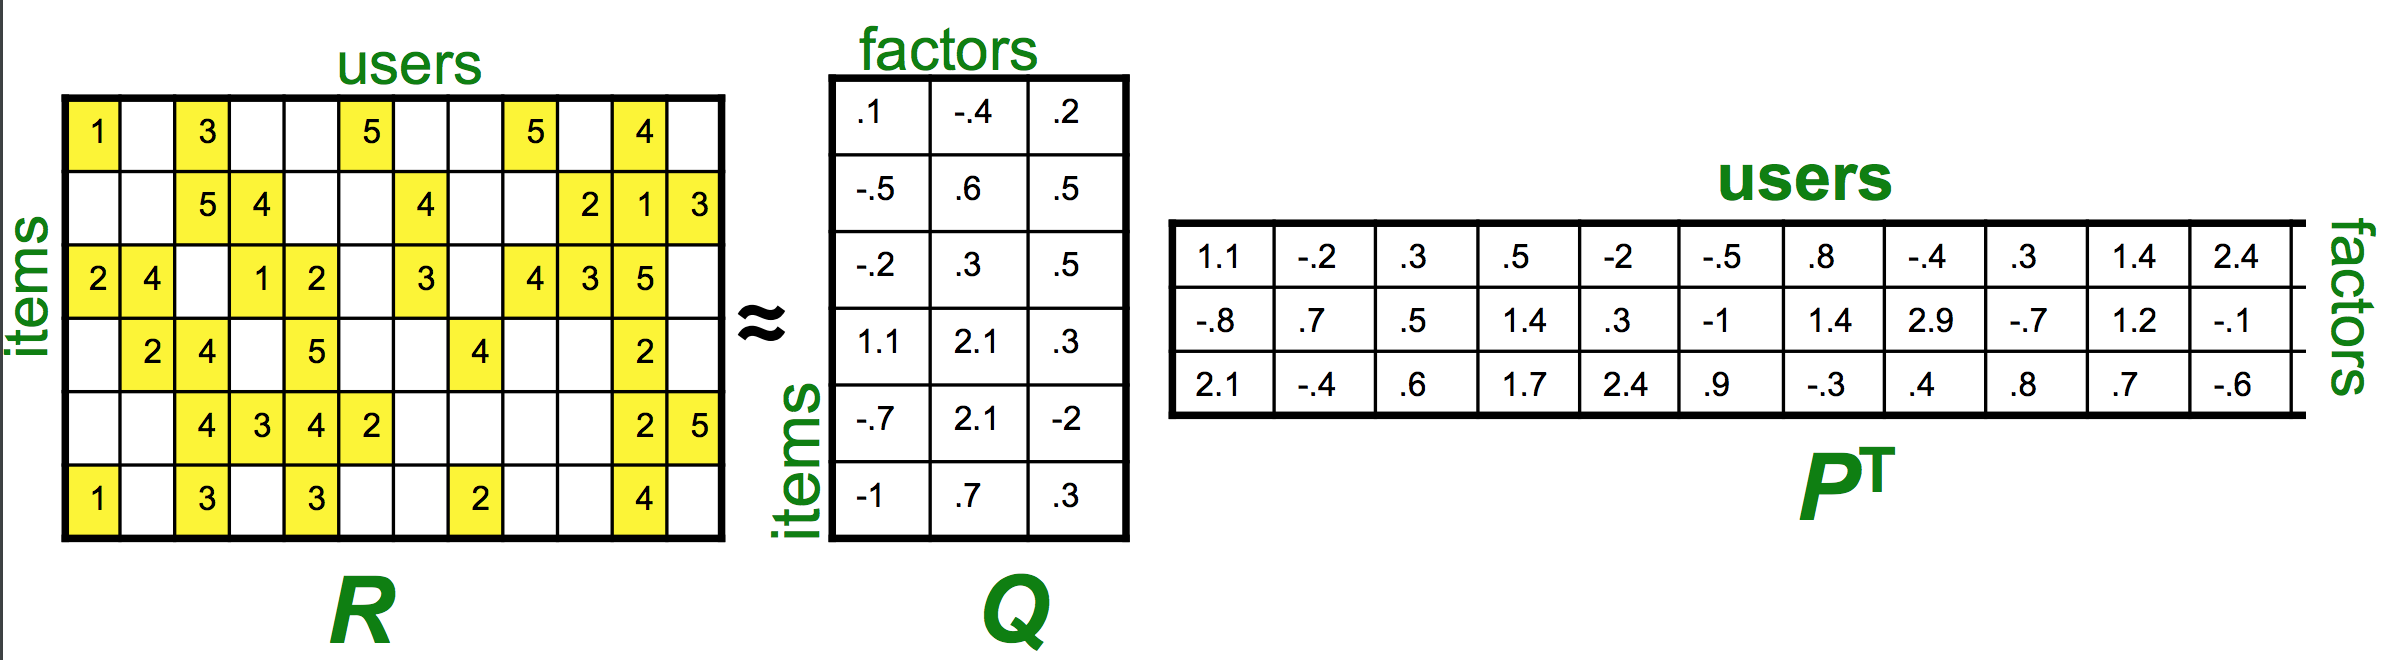
\includegraphics[width=0.9\textwidth]{cs246_model_m_factor}
\end{figure}
the scalar product of the dense factor of the users by the corresponding dense factor of the product  this will be a good approximation for the rating the user would give that product.

The problem of the approximation can be posed as a minimization problem. Let us define per each user $u \in \mathcal{U}$ a latent factor vector $\vec{x}_u \in \mathbb{R}^k$ and for each item  $i \in \mathcal{I}$ a latent factor $\vec{y}_i \in \mathbb{R}^k$. Then user predicted rating ($\hat{\cdot}$ denotes prediction) would be 
\begin{equation}
\hat{r}_{ui} = (\vec{x}_u, \vec{y}_i)
\end{equation}
In this setting the functional of choice to minimize would be :
\begin{equation}
\mathcal{L} = \sum_{u \in \mathcal{U}, i \in \mathcal{I}} 
\left\{r_{u,i}-(\vec{x}_u, \vec{y}_i)\right\} 
+ 
\lambda_u \sum_{\mathcal{U}}\norm{\vec{x}_u}^2
+ 
\lambda_i \sum_{\mathcal{U}}\norm{\vec{i}_i}^2
\end{equation}

\subsection{Explicit model. Alternative Least Squares}\label{eals}
For ALS procedure, one would proceed in a manner similar to stochastic gradient descent but a bit smarter. We iteratively would freeze one of the latent vectors and solve with respect to the others. For example one can start with item vectors. If items vectors are considered to be frozen, it is possible to  take the derivative of the loss function with respect to user latent vectors. Solving the equation given by the equating of the derivative to zero and freezing the variable makes it possible to proceed with {\it{alternative step}} and solve for the items. The process is repeated until convergence achieved \ref{On the Convergence of Alternating Least Squares Optimisation in Tensor Format Representations}
\begin{equation}
\frac{\partial \mathcal{L}}{\partial \vec{x}_u}  = -2 \sum_{i \in \mathcal{I}} \left(r_{u,i}-(\vec{x}_u, \vec{y}_i)\right) \vec{y}_i^T+
2\lambda_u \vec{x}_u^{T}
\end{equation}
Setting derivative to zero leads to 
\begin{equation}
\vec{x}_u^T  = \vec{r}_u\mathbb{Y}\left(\mathbb{Y}^T\mathbb{Y}+\lambda_u\mathbb{I}\right)^{-1}
\end{equation}


\section{Implicit Alternative Least Squares}\label{ials}
However the transactional data that is readily available in Oracle is implicit. The simplest way to treat the implicit feedback signals is to assume that a user  buying a product signals that user likes a product, the catch here is that with this approach there is no notion of a negative signal. Not having data does not mean that user does not like the product, it might simply indicate that user never encountered the product that otherwise might be of interest.

This means we can't just treat the missing data as unknowns, instead we have to treat a user not listening to an artist as being a signal that the user might not like that artist.

This presents a couple of challenges in learning a factorized representation.

The first challenge is in doing this factorization efficiently: by treating the unknowns as negatives, the naive implementation would look at every single entry in our input matrix. Since the dimensionality here is roughly 360K by 300K - there are over 100 billion total entries to consider, compared to only 17 million non zero entries.

The second problem is that we can't be certain that a user not listening to an artist actually means that they don't like it. There could be other reasons for the artist not being listened to, especially considering that we only have the top 50 most played artists for each user in the dataset.

The Collaborative Filtering for Implicit Feedback Datasets paper accounts for both of these challenges in an elegant way.

To handle the case where we're not confident about our negative data, this approach learns a factorized matrix representation using different confidence levels on binary preferences: unseen items are treated as negative with a low confidence, where present items are treated as positive with a much higher confidence.

The goal then is to learn user factors Xu and artist factors Yi by minimizing a confidence weighted sum of squared errors loss function:

\bibliographystyle{abbrv}
\bibliography{main}

\end{document}


-*/ßß¿¿???